\answer{Describe one key difference between client-server and peer-to-peer
applications.}{2}{2011.1.a}

P2p does not have a central point of coordination; all nodes are the same in
terms of functionality (though they may have different roles). A client server
architecture is dissimilar to this in the fact that the machines that make up
the network have different capabilities and responsibilities that cannot be
changed.

\answer{Explain briefly what failures are known as Byzantine failures and what
the Byzantine generals problem refers to.}{2}{2011.1.b}

Byzantine failures are ones where processes send failed messages since they are
malicious or faulty.

The Byzantine Generals problem refers to a situation where two generals  are
situated on the sides of a valley and want to attack a city in the valley. To
win the battle, they must attack at the same time, but they cannot coordinate
their attack with any guarantee of timing it properly since they can only send
messages through the city where the messengers may be killed or the contents of
the message changed.

\answer{Describe briefly the two-phase commit protocol.}{2}{2011.1.c}

\answer{Explain briefly why somebody would choose to use Cloud
Computing.}{2}{2011.1.d}

\answer{Why is it practically impossible to achieve strict consistency in a
distributed system?}{2}{2011.1.e}

It is practically impossible to achieve strict consistency in a distributed
system since latency is not zero, so you can never know exactly what is going on
in a remote system at any one time. Messages can get lost or mutated too, which
further complicates the sending and updating of state between systems.

\answer{Suppose the C function below is to be made available to remote processes
using RPC. What particular implementation problem does this highlight? Why
is the normal solution only partly satisfactory?}{2}{2011.1.f}

\begin{verbatim}
  void doIt (int *p, int *q) { (*p)++ ; (*q)-- ; return ; }
\end{verbatim}

You would have to serialise and deserialise the values of p and q to have this
function run over RPC, because it uses pointers as opposed to actual values. You
would also have to update the value of the pointers either as they are updated
during the RPC function’s execution or after the function has finished
executing.

\answer{Distinguish carefully between a name server and a directory
server.}{2}{2011.1.g}

A name server takes the name of a resource and resolves it into the address of
the resource (e.g. a URL). A directory server takes attributes about an object
(e.g. the amount of RAM of a server or the age and course studied of a student)
and returns information about objects that have the same attributes (think LDAP)

\answer{What is meant by the term causally ordered multicast?}{2}{2011.1.h}

Ummmmm? Maybe take a look here:
\url{http://www.cse.buffalo.edu/~stevko/courses/cse486/spring13/lectures/12-multicast2.pdf}

Looks like every process has a vector clock and when a message is received, the
process waits until it can preserve the causal ordering before accepting the
message. This means it waits until messages that had been previously sent to it
(according to the vector clock) arrive before accepting the new message. Until
then, the message is buffered.

\answer{What properties are provided by a secure channel? }{2}{2011.1.i}

A secure channel is one that third parties cannot eavesdrop on. They might be
able to see the data passing through, but it will be encrypted somehow so they
won’t be able to make sense of it.

\answer{The Andrew File System (AFS) uses callback promises. Explain what this
means.}{2}{2011.1.j}

Dunno? Google turns up not much...

I’m guessing that it is a mechanism where if you send a remote server a message,
it promises to reply back to you and will cause a callback to execute in your
code when it does.

\newpage

\answer{Explain briefly why some applications are not parallelisable. Describe
Amdahl’s law and explain what it can be used for.}{3}{2011.2.a}

Some applications are not parallelisable because they have operations that are
interdependent. For example, if we were building a machine to compute how long
it takes for the collatz conjecture to reach 1 given an input number, we could
not parallelise it since each stage of the conjuncture depends on the last.
Amdahl’s law dictates how much we can speed up the execution of a program given
how much of the program is parallelisable. The law is:

\[
  \frac{1}{\text{serial portion} + (\frac{1}{\text{num threads}} \times \text{parallel portion})}
\]

\answer{Explain briefly what the four properties commonly denoted by the acronym
ACID are when referring to transactions.}{3}{2011.2.b}

ACID stands for:
\begin{description}
  \item \textit{Atomic} - All or nothing principle; either the transaction is
  committed and its changes are applied, or no state is changed as a result of
  the transaction.

  \item \textit{Consistent} - Each transaction moves the system from one valid
  and consistent state to another.

  \item \textit{Isolated} - Each transaction executes independently from all
  other transactions (even if they may be happening concurrently). The effect of
  transactions in progress is hidden from all other transactions.

  \item \textit{Durable} - Once a transaction is committed, it stays committed
  even in the event of failure such as power loss etc
\end{description}

\answer{A service is replicated onto 3 computers.}{6}{2011.2.c}

\begin{itemize}
\item The first computer, A, has a mean time between failures of 2 days.
\item The second computer, B, has a mean time between failures of 3.5 days.
\item The third computer, C, has a mean time between failures of 12 days.
\end{itemize}

\textbf{When a failure occurs, it takes on average 12 hours to fix.}

\answer{What is the availability of the replicated service?}{2}{2011.2.c.i}

We need to find the chance that all the computers will fail at the same time.
It is easy to find the up-times for each individual computer:

\begin{description}
  \item A - $75\%$
  \item B - $85.7\%$
  \item C - $95.83\%$
\end{description}

The chance that these will all fail at the same time is:
$(1 - 0.75) * (1 - 0.875) * (1 - 0.9853) = 0.00046 = 0.046\%$
Therefore, the uptime is going to be $100 - 0.046 = 99.954\%$

\answer{What would the availability of the replicated service be if only
computers A and B were used?}{2}{2011.2.c.ii}

If only A and B were used, it would be:

$1 - ((1 - 0.75) * (1 - 0.875)) = 0.96875 = 96.88\%$

\answer{Describe how in the general case of n computers, each with a mean
time between failures $f_i$ and an average time to fix a failure $t_i$ you
would choose the two computers that provide the highest
availability.}{2}{2011.2.c.iii}

Rank the computers in ascending order of $t_x/f_x$, and take the top $n$
elements.

\answer{The following four processes access a shared variable x. Each process
accesses a different replica of the store used to hold this variable. Before any
process starts executing, the value of x is 0 in all the replicas.}{8}{2011.2.d}

\begin{center}
  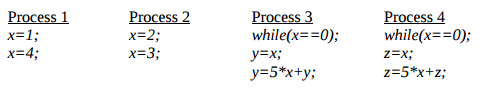
\includegraphics[width=0.5\textwidth]{images/2011-2-d}
\end{center}

\answer{When all four processes have completed executing the statements
given, are 7 and 14 possible values of y and z respectively, if the
replication uses the sequential consistency model? Justify your
answer.}{4}{2011.2.d.i}

With a sequential consistency model, it is not possible for the final values to
be $y=7$ and $z=14$, since for $y$ to equal $7$, $x$ must change state while
process $3$ is running, and this is not possible in a sequential consistency
model since only one process can execute at once.

The possible values of $x$ when process three actually starts are $x=4$ and
$x=3$, none of which let $y=7$.

\answer{When all four processes have completed executing the statements
given, are 7 and 14 possible values of y and z respectively, if the
replication uses the causal consistency model? Justify your
answer.}{4}{2011.2.d.ii}

Using a causal consistency model, we still can't get $y=7, z=14$, since we need
$y = 5 \times (x = 1) + (y = 2)$ and $z = 5 \times (x = 2) + (z = 4)$, but this
can never happen, since for $z = 4$, we need to have done $x = 1$, but  we need
to have done $y = 2$ before that, which means that we would have already done $x
= 2$.

\newpage

\answer{Describe in detail the Bully algorithm for the election of a leader in a
distributed system.}{8}{2011.3.a.i}

The Bully Algorithm works like this:

\begin{itemize}
\item An initiating client will send a message to all other clients with a
higher identifier than itself.
\item Any client receiving an election message will then start its own 
election, sending messages to clients with higher identifiers than itself.
\item Only when a process gets no replies (within a timeout) is it considered
elected. It then sends a message to all other processes announcing its election.
\end{itemize}

In this manner, any process that receives a message should always send a message
back to the sender

\answer{Carefully explain all the assumptions made in the Bully
algorithm.}{4}{2011.3.a.ii}

\begin{itemize}
  \item The timeouts are reasonable
  \item All processes know about all other processes (and their loads)
  \item Messages are delivered quickly
  \item Messages are delivered reliably
\end{itemize}

\answer{Describe one application for which the Bully algorithm might be applied,
indicating why a leader is needed.}{2}{2011.3.b}

In a peer-to-peer protocol (such as bit torrent), the Bully algorithm can be
used to elevate a node to coordinator status if the client that was coordinating
the network went offline or started to get a too high load.

\answer{In a system containing 6 computers, identified by the integers 1-6, the
leader is chosen by the Bully algorithm to be the live one with the highest
identifier. Assume for this part that all messages are delivered promptly, and
that the computers and the network are entirely reliable.}{6}{2011.3.c}

\answer{How many messages in total are sent so that the computer with
identifier 1 after it is rebooted can learn the identity of the leader by
triggering an election? Take care to explain your working!}{6}{2011.3.c.i}

Since identifier 1 is the lowest node, it will exhibit worst case behaviour for
the bully algorithm, $O(n^2)$.

This is because 1 will send five messages out (to each other process) to start
the election. Client 2 will then send out four messages (to the ones bigger than
it) etc, until there are $5 + 4 + 3 + 2 + 1 + 0 = 15$ messages sent. Since every
client receiving an election message replies to the sender, then $15$ replies
will be sent (in addition to the 15 initial message). Then, the winner of the
election (6) will send a message out to say that it is elected, which is another
$5$ messages, bringing the total to 35.

\answer{Repeat (i) with the computer rebooted and needing to discover the leader
being that with identifier 5 instead.}{2}{2011.3.c.ii}

If 6 wasn't online anymore, then the number of messages sent would be $(5 + 4 +
3 + 2 + 1) + (4 + 3 + 2 + 1) + 4 = 29$,
